\documentclass{beamer}
\usepackage{luatexja} 
\usepackage[ipaex]{luatexja-preset} 
\renewcommand{\kanjifamilydefault}{\gtdefault}

\usepackage{bm} %bold → \mathbf{}
\usepackage{mathtools} 
\usepackage{amsmath} 
\usepackage{amsthm}
\usepackage{setspace}
\usepackage{graphicx}

\newtheorem{thm}{Theorem}[section] 
\newtheorem{lem}[thm]{Lemma} 
\newtheorem{prop}[thm]{Proposition} 
\newtheorem{assumption}[thm]{Assumption} 
\usetheme{PaloAlto} 
\usecolortheme{dove}
\setbeamertemplate{navigation symbols}{} 

\DeclareMathOperator*{\argmax}{arg\,\max}
\DeclareMathOperator*{\argmin}{arg\,\min}
\renewcommand{\baselinestretch}{0.95}

%\newcommand{\relmiddle}[1]{\mathrel{}\middle#1\mathrel{}}% resized \mid → relmiddle |

\title{Heterogeneous impacts of informal caregiving on labor market outcomes:} 
\subtitle{Research Proposal}
\author{M1 Inoue Jin}
\institute{Hitotsubashi University} 
\date{2022/10/31}


\begin{document}

\begin{frame}
    \titlepage
\end{frame}

\begin{frame}{Outline}
    \tableofcontents
\end{frame}

\section{Introduction}
    \subsection{Why does informal caregiving matter?}
        \begin{frame}\frametitle{Why does informal caregiving matter?}
            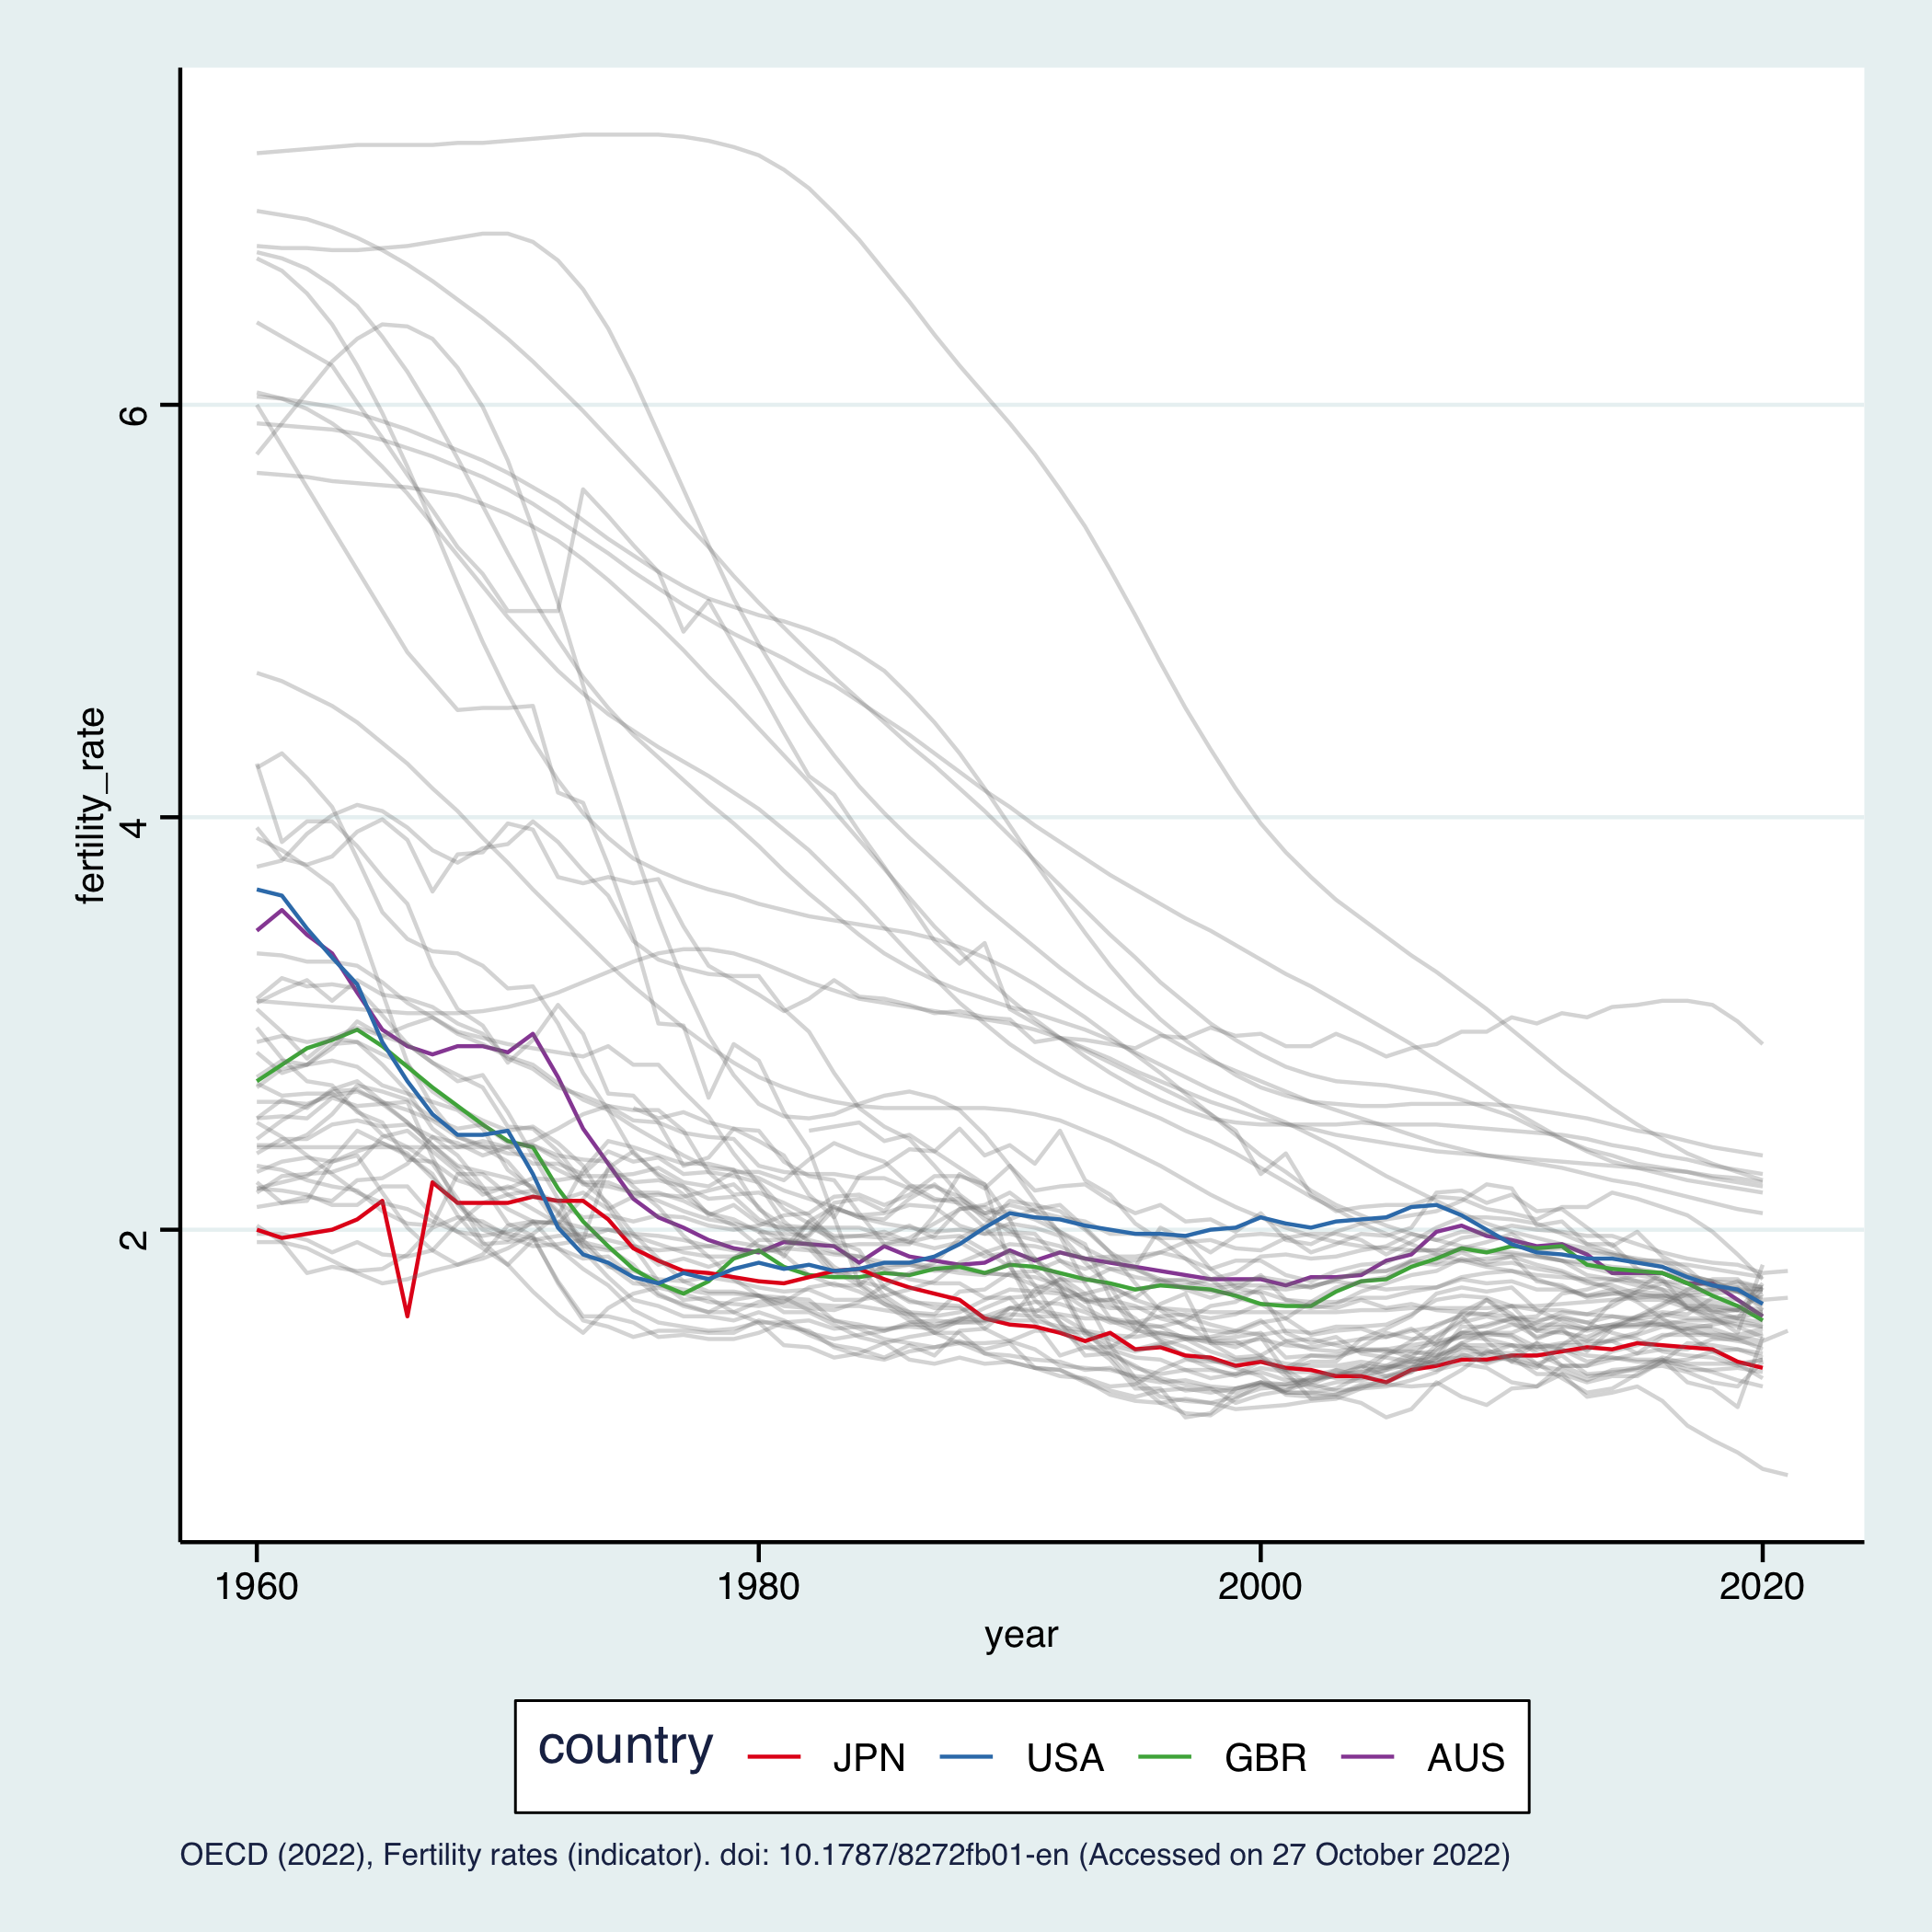
\includegraphics[height = 5cm]{OECD_fertility_rates.png}
            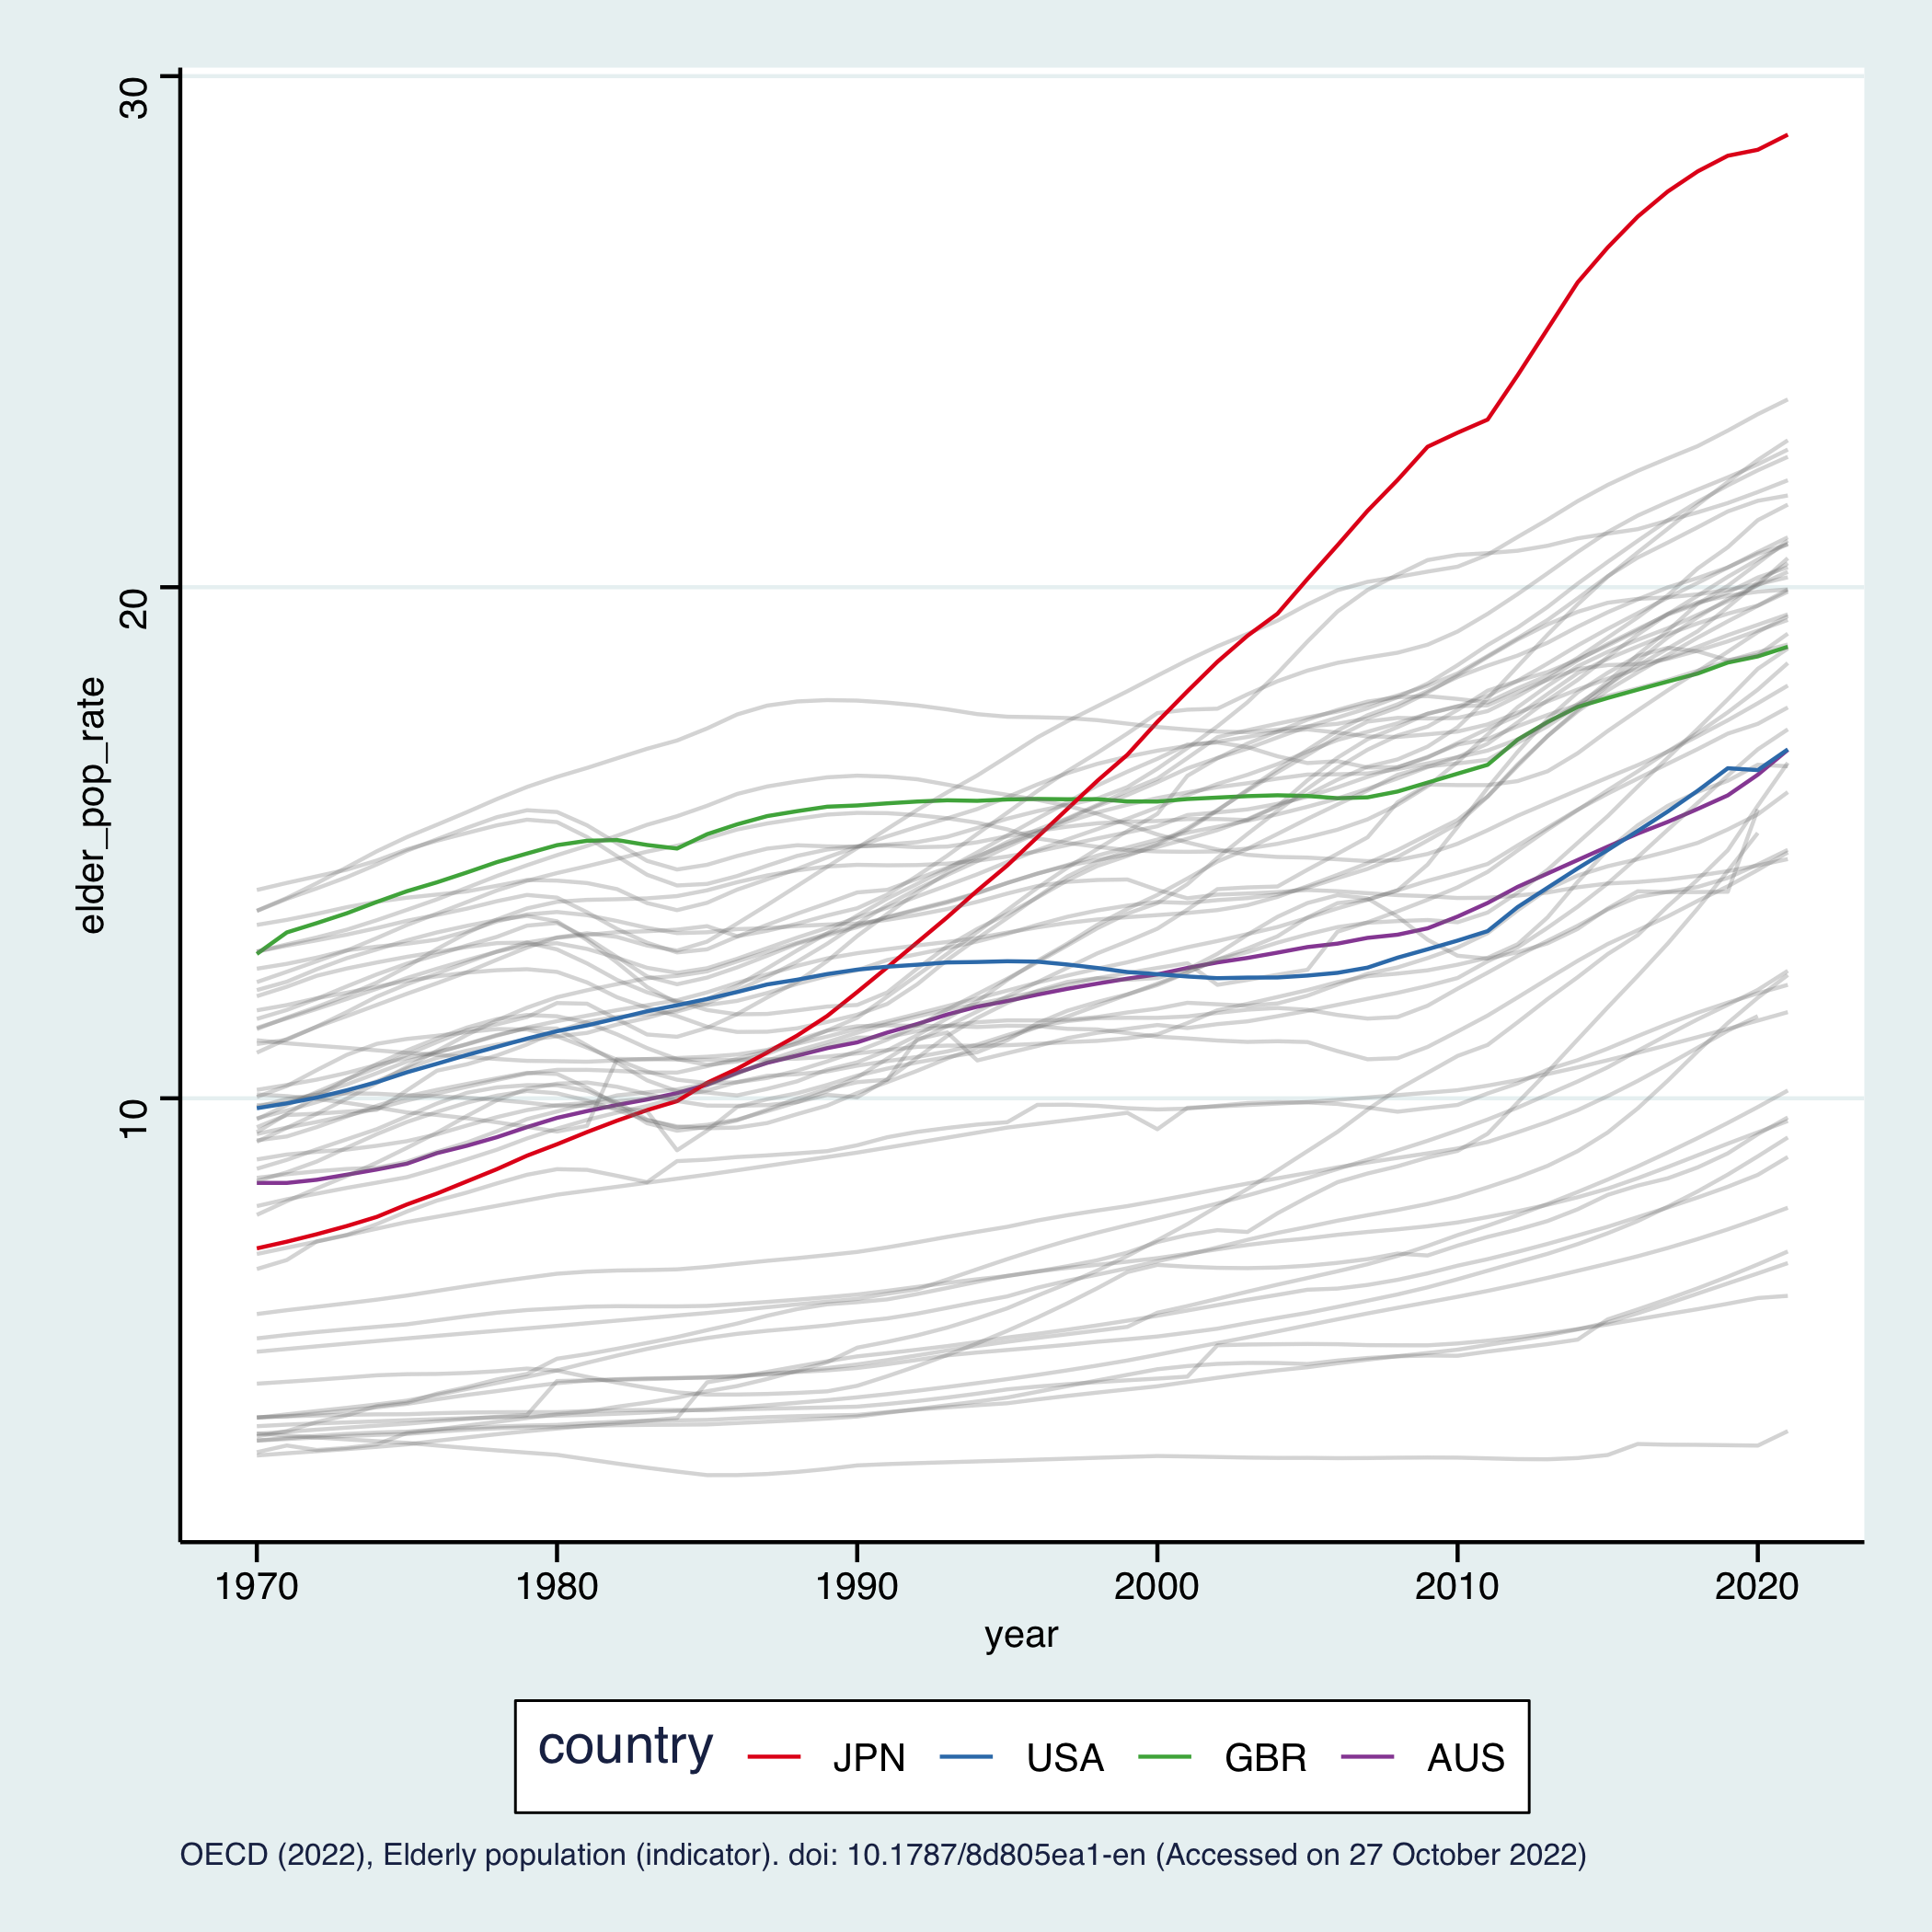
\includegraphics[height = 5cm]{OECD_Elderly_pop_rate.png}
            \begin{itemize}
                \item Most of developed countries are facing with the decline of fertility rates and experiencing aging society.
                \item These trends predict that the supply of labor markets will decrease in the long run while the demand for caregiving will continue to increase. 
            \end{itemize}
        \end{frame}
        \begin{frame}\frametitle{Why does informal caregiving matter?}
            \begin{itemize}
                \item Care-givers face a trade-off between hours of work, leisure and time for care-giving.
                \item Intuitively, there seems to be an negative relationship between care-giving and one's employment and hours of work. But empirically, it's not obvious whether care-givers have negative effects on  one's employment and hours of work.  
            \end{itemize}
        \end{frame}
        \begin{frame}\frametitle{Why does informal caregiving matter?}
            \begin{center}
            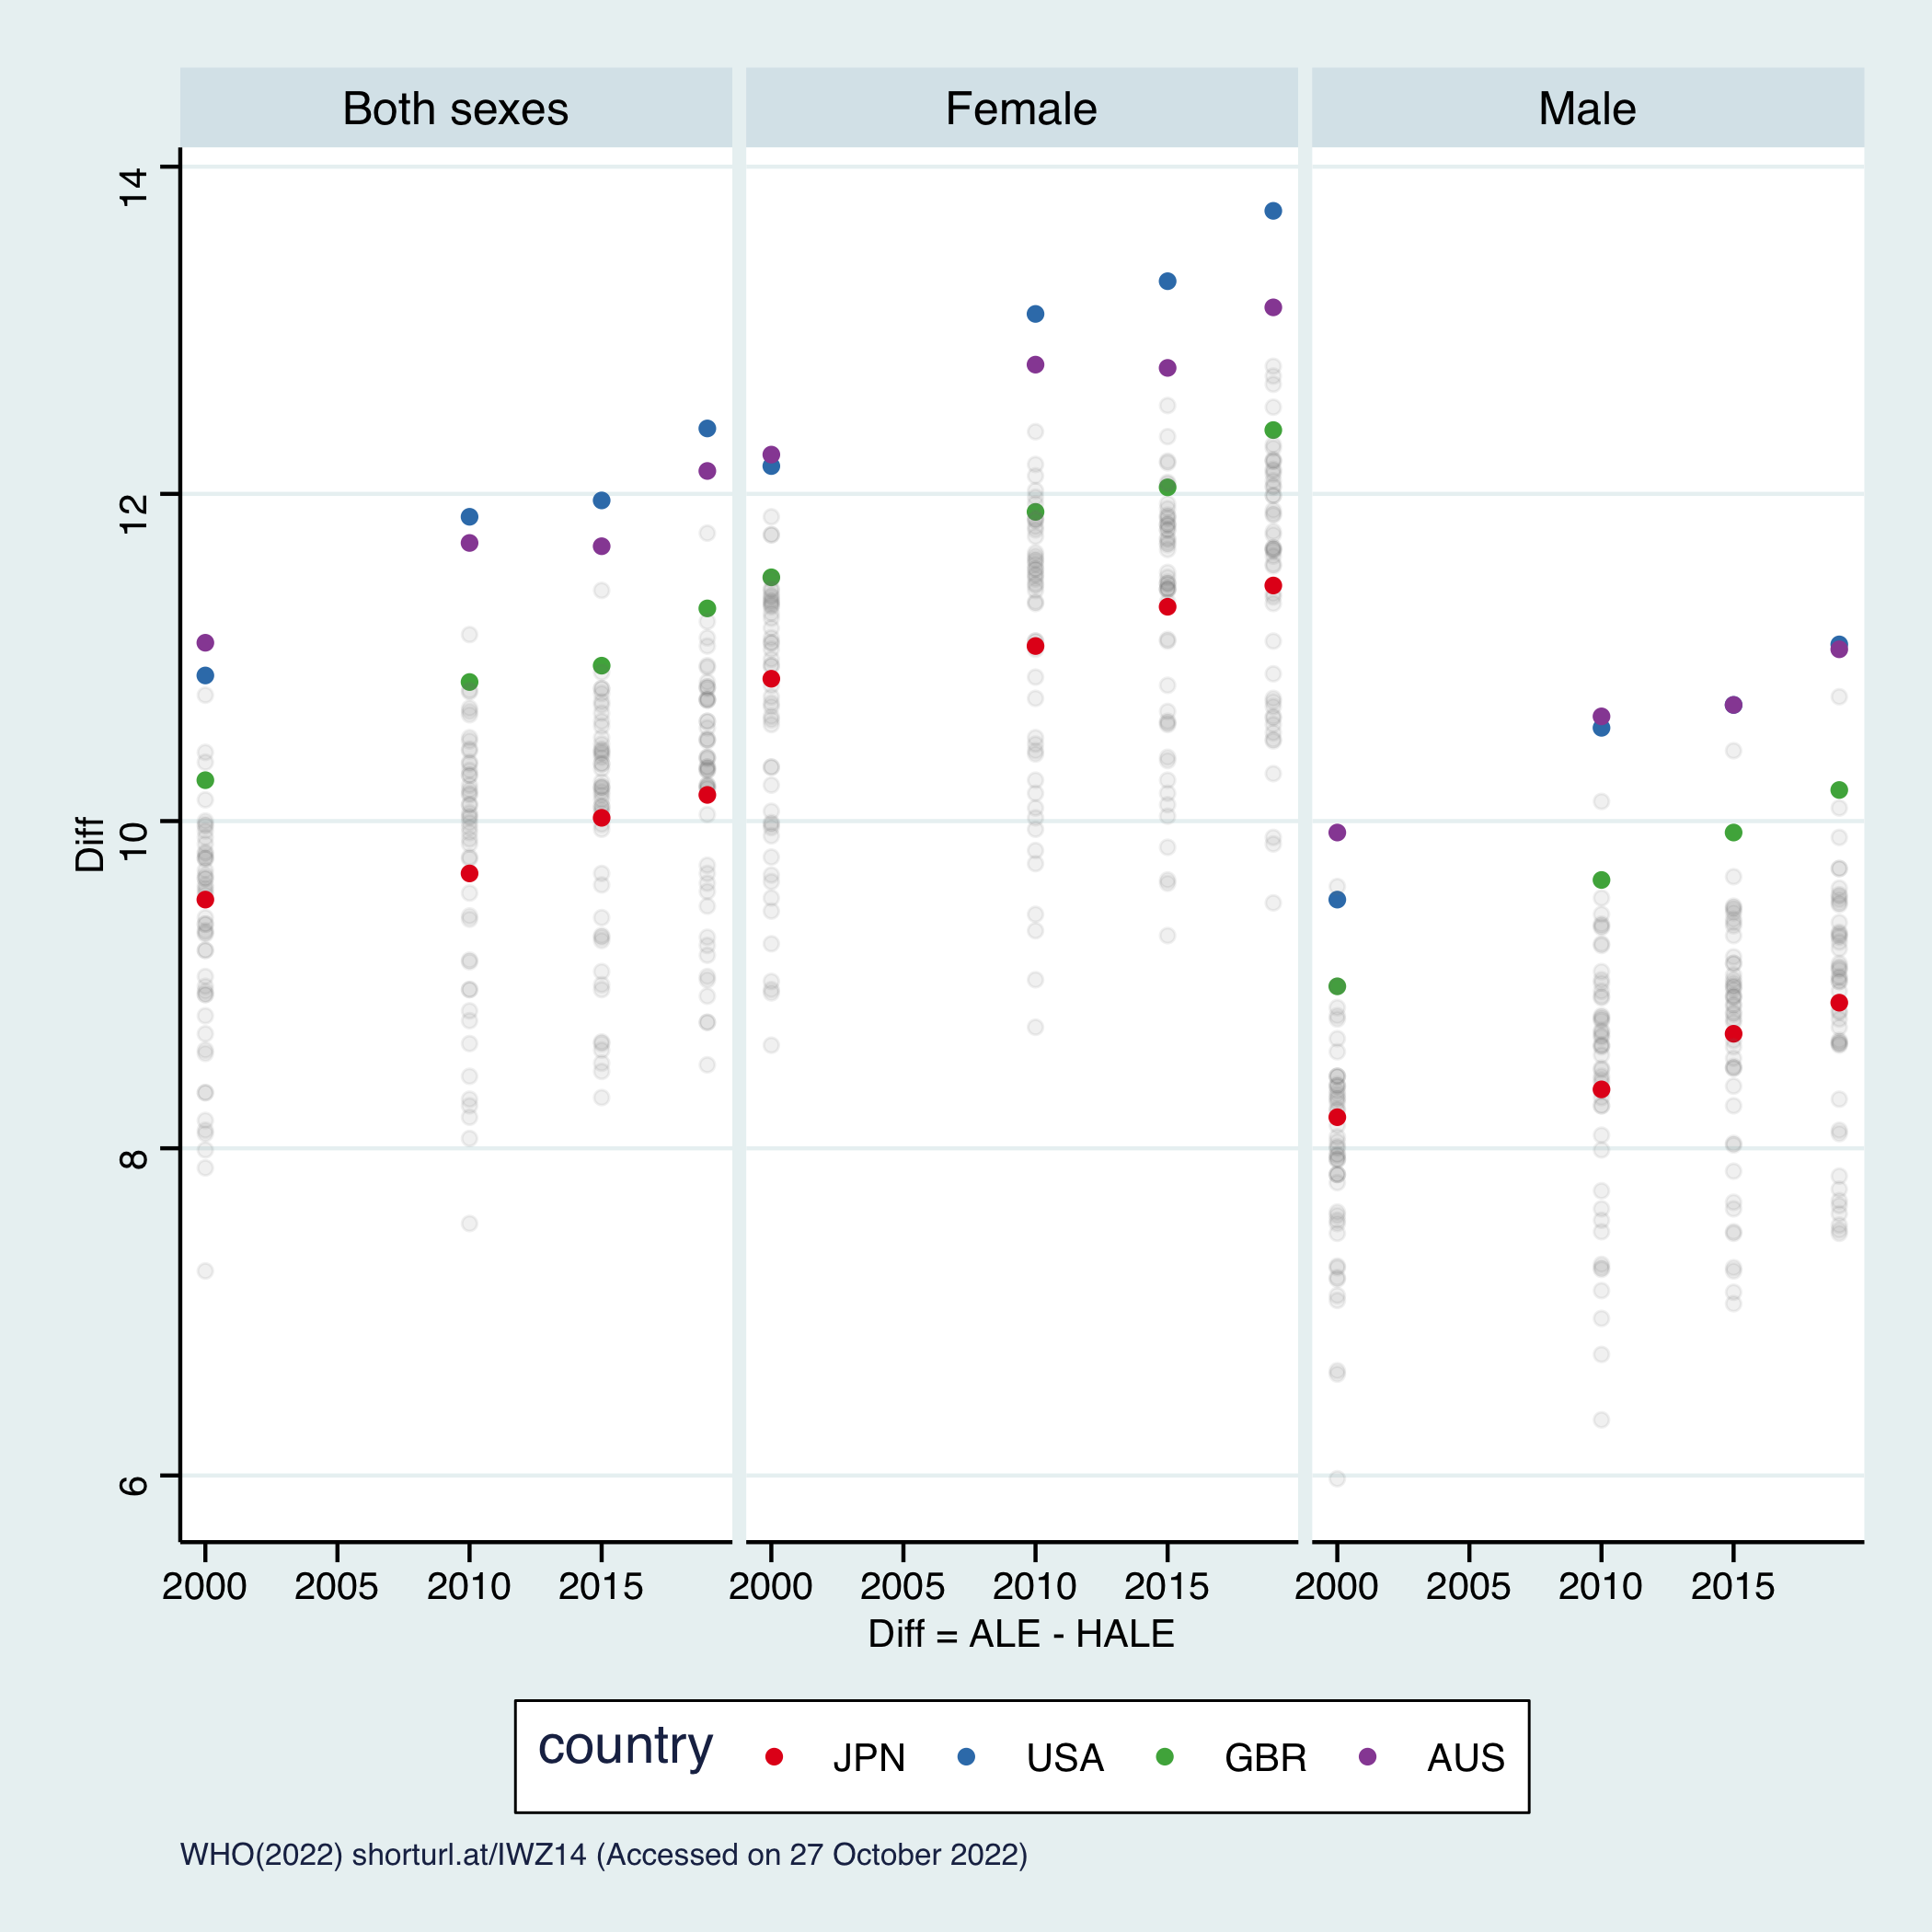
\includegraphics[width = 5.5cm]{WHO_diff_expectancy.png}
            \end{center}
            \begin{itemize}
                \item ALE = (Average) Life Expectancy
                \item HALE = Healthy Life Expectancy
                \item Difference of ALE and HALE is the expected length of years one needs care in some way.
            \end{itemize}
        \end{frame}
    \subsection{Literature review}
        \begin{frame}\frametitle{Literature review}
            \begin{itemize}
                \item Almost all the literature show the negative estimates
            \end{itemize}
        \end{frame}
    \subsection{Summary}

\section{Data}
\section{Problems related with estimation}
    \subsection{Negative weights and negative effects may produce positive bias.}
    \subsection{Time-heterogeneous treatment effects should be evaluated.}
\section{Discussion:Remaining problems}
\section{References}

\begin{frame}\frametitle{Expected Contributions of this project}
    \begin{itemize}
        \item Suspecting previous literature using fixed effect estimation underestimate the absolute size of the effect. 
        \item There may be some heterogeneity of effects in terms of the various lengths of the treatment.
    \end{itemize}
\end{frame}



\end{document}




